\section{Robust Minimal Recursion Semantics}
\label{sec:rmrs}

We will now make the basic ideas from Section \ref{sec:motivation}
precise.  We will first define the syntax of the \rmrs\ language; this
is a notational variant of earlier definitions in the literature.  We
will then define a model theory for our version of \rmrs, and conclude
this section by carrying over the notion of \emph{solved forms} from
{\sc clls} \cite{egg:etal:2001}.



\subsection{RMRS Syntax}

We define \rmrs\ syntax in the style of {\sc clls}
\cite{egg:etal:2001}.  We assume an infinite set of {\em node
  variables} $\nvar=\{X,Y,X_1,\ldots\}$, used as labels, anchors, and
holes; the distinction between these will come from their
position in the formulas.  We also assume an infinite set of
\emph{base variables} $\ovar$, consisting of individual variables
$\{x,x_1,y,\ldots\}$ and event variables $\{e_1,\ldots\}$, and a
vocabulary of \emph{predicate symbols}
$\pred=\{P,Q,P_1,\ldots\}$.
\rmrs\ formulas are defined as follows.

\begin{definition}\label{defn:rmrs-syntax}
  An \emph{\rmrs} is a finite set $\varphi$ of atoms of one of the
  following forms; $S \subseteq \N$ is a set of numbers that is either
  finite or $\N$ itself (throughout the paper, we assume 
    $0 \in \N$).

$\begin{array}{rrll}
A &::= &\ep{X}{Y}{P} \\ %& \mbox{labelled elementary predication} \\
&| &\ARG_S(X,v) \\ % & \mbox{ARG relation for base variables} \\
&| &\ARG_S(X,Y) \\ % & \mbox{ARG relation for node variables} \\
&| &X \dom Y \\ % & \mbox{dominance} \\
&| &v_1 = v_2 \;|\; v_1 \neq v_2 \\ % & \mbox{base variable
                                % (in)equality} \\
&| &X = Y \;|\; X \neq Y \\ % & \mbox{node variable (in)equality} \\
&| &P \spec Q % & \mbox{SPEC relation between predicate symbols}
\end{array}
$

A node variable $X$ is called a \emph{label} iff $\varphi$ contains an
atom of the form $\ep{X}{Y}{P}$ or $Y \dom X$; it is an 
\emph{anchor} iff $\varphi$ contains an atom
of the form $\ep{Y}{X}{P}$ or $\ARG_S(X,i)$; and it is a
\emph{hole} iff $\varphi$ contains an atom of the form $\ARG_S(Y,X)$
or $X \dom Y$.
\end{definition}

Def.~\ref{defn:rmrs-syntax} combines similarities to earlier
presentations of \rmrs\ \cite{copestake:2003,copestake:2007b} and to
{\sc clls}/dominance constraints \cite{egg:etal:2001}.  For the most
part, our syntax generalises that of older versions of \rmrs: We use
$\ARG_{\{i\}}$ (with a singleton set $S$) instead of $\ARG_i$ and
$\ARG_\N$ instead of $\ARG_n$, and the {\sc ep} $\ep{l}{a}{P(v)}$ (as
in Section~\ref{sec:motivation}) is an abbreviation of
$\{\ep{l}{a}{P}, \ARG_{\{0\}}(a,v)\}$.  Similarly, we don't assume
that labels, anchors, and holes are syntactically different objects;
they receive their function from their positions in the formula.  One
major difference is that we use dominance ($\dom$) rather than qeq; see
Section~\ref{sec:extensions} for a discussion.  Compared to dominance
constraints, the primary difference is that we now have a mechanism
for representing lexical ambiguity, and we can specify a predicate and
its arguments separately.


\subsection{Model Theory} \label{sec:model-theory}

The model theory formalises the relationship between an {\sc rmrs} and
the fully specific, alternative logical forms that it describes,
expressed in the base language.  We represent such a logical form as a
tree $\tau$, such as the ones in Fig.~\ref{fig:1}, and we can then
define satisfaction of formulas in the usual way, by taking the tree
as a model structure that interprets all predicate symbols specified
above.

In this paper, we assume for simplicity that the base language is as
in \mrs; essentially, $\tau$ becomes the structure tree of a formula
of predicate logic.  We assume that $\Sigma$ is a ranked signature
consisting of the symbols of predicate logic: a unary constructor
$\neg$ and binary constructors $\wedge$, $\rightarrow$, etc.; a set of
3-place quantifier symbols such as $\sem{\_every\_q\_1}$ and
$\sem{\_some\_q\_1}$ (with the children being the bound variable, the
restrictor, and the scope); and constructors of various arities for
the predicate symbols; e.g., $\sem{\_chase\_v\_1}$ is of arity 3.
Other base languages may require a different signature $\Sigma$ and/or
a different mapping between formulas and trees; the only strict
requirement we make is that the signature contains a binary
constructor $\wedge$ to represent conjunction.  We write $\Sigma_i$
and $\Sigma_{\geq i}$ for the set of all constructors in $\Sigma$ with
arity $i$ and at least $i$, respectively.  We will follow the
typographical convention that non-logical symbols in $\Sigma$ are
written in \textsf{sans-serif}, as opposed to the \rmrs\ predicate
symbols like $\sempred{\_cat\_n}$ and $\sempred{\_cat\_n\_1}$.

The models of {\sc rmrs} are then defined to be finite constructor
trees (see also \cite{egg:etal:2001}):
\begin{definition}\label{defn:models}
  A {\em finite constructor tree} $\tau$ is a function $\tau:D
  \rightarrow \Sigma$ such that $D$ is a \emph{tree domain} (i.e., a
  subset of $\N^*$ which is closed under prefix and left sibling) and
  the number of children of each node $u \in D$ is equal to the arity
  of $\tau(u)$.  
\end{definition}

We write $D(\tau)$ for the tree domain of a constructor tree $\tau$,
and further define the following relations between nodes in a finite
constructor tree:

\begin{definition}\label{defn:dominance}
  $u \dom v$ \emph{(dominance)} iff $u$ is a prefix of $v$, i.e.\ the node
  $u$ is equal to or above the node $v$ in the tree.
  $u \wedgedom v$ iff $u \dom v$, and all symbols on the path from $u$
  to $v$ (not including $v$) are $\wedge$.
\end{definition}

The {\em satisfaction} relation between an \rmrs\ $\varphi$ and a
finite constructor tree $\tau$ is defined in terms of several
assignment functions.  First, a node variable assignment
function $\alpha: \nvar \rightarrow D(\tau)$ maps the node
variables in an \rmrs\ to the nodes of $\tau$.  Second, a
base language assignment function $g:\ovar \rightarrow \Sigma_0$ 
maps the base variables to nullary constructors
representing variables in the base language. Finally, a
relation $\sigma \subseteq \pred \times \Sigma_{\geq 1}$ maps
each \rmrs\ predicate symbol to a set of constructors from $\Sigma$.
As we'll see shortly, this relation allows an \rmrs\ to underspecify lexical
ambiguities.

\begin{definition}\label{defn:satisfaction}
Satisfaction of atoms is defined as follows:
$$
\begin{array}{l}
  \tau, \alpha, g, \sigma \models  \ep{X}{Y}{P}
\mbox{ iff}\\
\qquad \tau(\alpha(Y)) \in \sigma(P) \mbox{ and } \alpha(X) \wedgedom
  \alpha(Y) \\
  \tau, \alpha, g, \sigma \models \ARG_S(X,a)
\mbox{ iff exists  $i \in S$ s.t.}\\
\qquad  \alpha(X) \cdot i \in D(\tau) \mbox{ and }
  \tau(\alpha(X) \cdot 
  i) = g(a) \\
  \tau, \alpha, g, \sigma \models \ARG_S(X,Y)
\mbox{ iff  exists $i \in S$ s.t.}\\
\qquad \alpha(X) \cdot i \in D(\tau), \alpha(X) \cdot
  i = \alpha(Y)\\
  \tau, \alpha, g, \sigma \models X \dom Y
\mbox{ iff } \alpha(X) \dom \alpha(Y) \\
  \tau, \alpha, g, \sigma \models X =  \!\!/\!\! \neq Y
\mbox{ iff }  \alpha(X) =  \!\!/\!\! \neq \alpha(Y) \\
  \tau, \alpha, g, \sigma \models v_1 =  \!\!/\!\! \neq v_2
\mbox{ iff }  g(v_1) = \!\!/\!\! \neq g(v_2) \\
  \tau, \alpha, g, \sigma \models P \spec Q
\mbox{ iff $\sigma(P) \subseteq \sigma(Q)$}
\end{array}
$$
A 4-tuple $\tau,\alpha,g,\sigma$ satisfies an \rmrs\ $\varphi$
(written $\tau,\alpha,g,\sigma \models \varphi$) iff it satisfies all
of its elements.
\end{definition}

Notice that one \rmrs\ may be satisfied by multiple trees; we can take
the \rmrs\ to be a partial description of each of these trees.  In
particular, \rmrs s may represent semantic scope ambiguities and/or
missing information about semantic dependencies, lexical
subcategorisation and lexical senses.  For $j=\{1,2\}$, suppose that
$\tau_j,\alpha_j,g_j,\sigma\models \varphi$.  Then $\varphi$ exhibits
a semantic scope ambiguity if there are variables $Y,Y'\in \nvar$ such
that $\alpha_1(Y) \dom \alpha_1(Y')$ and $\alpha_2(Y')\dom
\alpha_2(Y)$.  It exhibits missing information about semantic
dependencies if there are base-language variables $v,v'\in \ovar$ such
that $g_1(v)=g_1(v')$ and $g_2(v)\neq g_2(v')$.  It exhibits missing
lexical subcategorisation information if there is a $ Y \in \nvar$
such that $\tau_1(\alpha_1(Y))$ is a constructor of a different type
from $\tau_2(\alpha_2(Y))$ (i.e., the constructors are of a different
arity or they differ in whether their arguments are scopal vs.\
non-scopal).  And it exhibits missing lexical
sense information if $\tau_1(\alpha_1(Y))$ and $\tau_2(\alpha_2(Y))$
are different base-language constructors, but of the same type.

Let's look again at the \rmrs\ (\ref{ex:cat-pos}).
This is satisfied by the trees in Fig.~\ref{fig:1} (among
others) together with some particular $\alpha$, $g$, and $\sigma$.
For instance, consider the left-hand side tree in Fig.~\ref{fig:1}.
The \rmrs\ (\ref{ex:cat-pos}) satisfies this tree with an assignment
function $\alpha$ that maps the variables $l_1$ and $a_1$ to the root
node, $l_{41}$ and $l_{42}$ to its second child (labeled with
``$\wedge$''), $a_{41}$ to the first child of \emph{that} node (i.e.\
the node 21, labelled with ``fat'') and $a_{42}$ to the node 22, and
so forth.  $g$ will map $x_1$ and $x_3$ to $x$, and $x_6$ and $x_7$ to
$y$, and so on.  And $\sigma$ will map each \rmrs\ predicate symbol
(which represents a word) to the set of its fully resolved meanings, e.g.\
\_cat\_n to a set containing $\sem{\_cat\_n\_1}$ and possibly others.
It is then easy to verify that every single atom in the \rmrs\ is
satisfied---most interestingly, the {\sc ep}s
$\ep{l_{41}}{a_{41}}{\sempred{\_fat\_j}(e')}$ and
$\ep{l_{42}}{a_{42}}{\sempred{\_cat\_n}(x_3)}$ are satisfied because
$\alpha(l_{41}) \wedgedom \alpha(a_{41})$ and $\alpha(l_{42})
\wedgedom \alpha(a_{42})$.

Truth, validity and entailment can now be defined in terms of
satisfiability in the usual way:
\begin{definition}\label{defn:entailment}
\begin{description}
\item   [truth:] $\tau\models \varphi$ iff $\exists \alpha,g,\sigma$  such
  that $\tau,\alpha,g,\sigma\models \varphi$
\item   [validity:] $\models \varphi$ iff $\forall \tau$, $\tau\models \varphi$.
\item   [entailment:] $\varphi\models \varphi'$ iff $\forall \tau$, if
  $\tau\models \varphi$ then $\tau\models \varphi'$.
\end{description}
\end{definition}
% NOTE: This definition of entailment isn't right, because it allows
% the assignment $\sigma$ from predicates to constructors to vary
% when testing the satisfiability of $\varphi$ vs. $\varphi'$ with
% respect to $\tau$.  I think that to get the notion of entailment we
% want, $\sigma$ should actually be part of the {\sc rmrs} *model*.
% In other words, an {\sc rmrs} model $M$ is a tuple $\langle \tau,
% \sigma\rangle$, where $\tau$ is a finte constructor tree and
% $\sigma$ is a mapping from $\Pred$ to the power set of $\Sigma$.
% Then truth and entailment are defined correctly.  I believe our
% proofs of things like Theorem~\ref{thm:big-one} actually assumes
% that $\sigma$ is constant when interpreting $\varphi$ vs.\
% $\varphi'$, no?



\subsection{Solved Forms}

One aspect in which our definition of \rmrs\ is like dominance
constraints and unlike \mrs\ is that any satisfiable \rmrs\ has an
infinite number of models which only differ in the areas that the
\rmrs\ didn't ``talk about''.  Reading (\ref{ex:cat-erg})
as an \mrs\ or as an \rmrs\ of the previous literature, this
formula is an instruction to build a semantic representation out of
the pieces for ``every fat cat'', ``some dog'', and ``chased''; a
semantic representation as in Fig.~\ref{fig:fat-black-cat} would
\emph{not} be taken as described by this \rmrs.  However, under the
semantics we proposed above, this tree is a correct model of
(\ref{ex:cat-erg}) because all atoms are still satisfied; the \rmrs\
didn't say anything about ``sleep'' or ``run'', but it couldn't
enforce that the tree shouldn't contain those subformulas either.

\begin{figure}
  \centering
  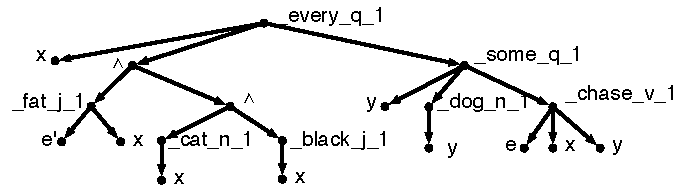
\includegraphics[width=\columnwidth]{pic-more-stuff}
  \caption{Another tree which satisfies (\ref{ex:cat-erg}).}
  \label{fig:fat-black-cat}
\end{figure}

In the context of robust semantic processing, this is a desirable
feature, because it means that when we enrich an \rmrs\ obtained from
a shallow processor with more semantic information---such as the
relation symbols introduced by syntactic constructions such as
appositives, noun-noun compounds and free adjuncts---we don't change
the set of models; we only \emph{restrict} the set of models further
and further towards the semantic representation we are trying to
reconstruct.  Furthermore, it has been shown in the literature that a
dominance-constraint style semantics for underspecified
representations gives us more room to manoeuvre when developing
efficient solvers than an \mrs-style semantics
\cite{Althaus_etal:JoA}.

However, enumerating an infinite number of models is of course
infeasible.  For this reason, we will now transfer the concept of
\emph{solved forms} from dominance constraints to \rmrs.  An \rmrs\ in
solved form is guaranteed to be satisfiable, and thus each solved form
represents an infinite class of models.  However, each satisfiable
\rmrs\ has only a finite number of solved forms which partition the
space of possible models into classes such that models within a class
differ only in `irrelevant' details.  A solver can then enumerate the
solved forms 
rather than all models.

Intuitively, an \rmrs\ in solved form is fully
specified with respect to the predicate-argument structure, all
variable equalities and inequalities and scope ambiguities have been
resolved, and only lexical sense ambiguities remain.  This is made
precise below.

\begin{definition}\label{defn:solved-forms}
  An RMRS $\varphi$ is \emph{in solved form} iff:
  \begin{enumerate}
  \item every variable in $\varphi$ is either a hole, a label or an
    anchor (but not two of these);
  \item $\varphi$ doesn't contain equality, inequality, and SPEC
    ($\sqsubseteq$) atoms;
  \item if $\ARG_S(Y,i)$ is in $\varphi$, then $|S| = 1$;
  \item for any label $Y$ and index set $S$, there
    are no two atoms $\ARG_S(Y,i)$ and $\ARG_S(Y,i')$ in $\varphi$;
  \item if $Y$ is an anchor in some {\sc ep} $\ep{X}{Y}{P}$ and $k$ is the
    maximum number such that $\ARG_{\{k\}}(X,i)$ is in $\varphi$ for
    any $i$, then there is a constructor $p \in \sigma(P)$ whose arity
    is at least $k$;
  \item no label occurs on the right-hand side of two
    different $\dom$ atoms.
  \end{enumerate}
\end{definition}

Because solved forms are so restricted, we can `read off' at least one
model from each solved form:
\begin{prop} \label{prop:solved-forms-are-satisfiable}
  Every {\sc rmrs} in solved form is satisfiable.
\end{prop}
\begin{proof}[Proof (sketch; see also
  \cite{Duchier00dominanceconstraints})] 
  For each {\sc ep}, we choose to label the anchor with the
  constructor $p$ of sufficiently high arity whose existence we
  assumed; we determine the edges between an anchor and its children
  from the uniquely determined $\ARG$ atoms; plugging labels into
  holes is straightforward because no label is dominated by more than
  one hole; and spaces between the labels and anchors are filled with
  conjunctions.
\end{proof}


We can now define the solved forms \emph{of} an \rmrs\ $\varphi$;
these finitely many \rmrs s in solved form partition the space of
models of $\varphi$ into classes of models with trivial differences.

\begin{definition} \label{defn:solved-form-of} The \emph{syntactic
    dominance relation} $D(\varphi)$ in an {\sc rmrs} $\varphi$ is the
  reflexive, transitive closure of the binary relation $$
\begin{array}{r c l}
\{(X,Y) & \mid &  \mbox{$\varphi$ contains $X \dom Y$ or}\\
&& \mbox{$ARG_S(X,Y)$ for some
    $S$}\}
\end{array}
$$  


  An RMRS $\varphi'$ is \emph{a solved form of} the RMRS $\varphi$
  iff $\varphi'$ is in solved form and there is a substitution $s$
  that maps the  node and base variables of $\varphi$ to the node and
  base variables of $\varphi'$ such that
  \begin{enumerate}
  \item $\varphi'$ contains the {\sc ep} $\ep{X'}{Y'}{P}$ iff there are
    variables $X,Y$ such that $\ep{X}{Y}{P}$ is in $\varphi$, $X' =
    s(X)$, and $Y' = s(Y)$;
  \item for every atom $\ARG_S(X,i)$ in $\varphi$, there is exactly
    one atom $\ARG_{S'}(X',i')$ in $\varphi'$ with $X' = s(X)$, $i' =
    s(i)$, and $S' \subseteq S$;
  \item $D(\varphi') \supseteq s(D(\varphi))$.
  \end{enumerate}
\end{definition}

\begin{prop} \label{prop:models-satisfy-solved-forms}
  For every tuple $(\tau,\alpha,g,\sigma)$ that satisfies some \rmrs\
  $\varphi$, there is a solved form $\varphi'$ of $\varphi$ such that
  $(\tau,\alpha,g,\sigma)$ also satisfies $\varphi'$.
\end{prop}
\begin{proof}
  We construct the substitution $s$ from $\alpha$ and $g$.  Then we
  add all dominance atoms that are satisfied by $\alpha$ and restrict
  the $\ARG$ atoms to those child indices that are actually used in
  $\tau$.  The result is in solved form because $\tau$ is a tree; it
  is a solved form of $\varphi$ by construction.
\end{proof}

\begin{prop}  \label{prop:finite-solved-forms}
  Every {\sc rmrs} $\varphi$ has only a finite number of solved forms, up to
  renaming of variables.
\end{prop}
\begin{proof}
  Up to renaming of variables, there is only a finite number of
  substitutions on the node and base variables of $\varphi$.  Let $s$
  be such a substitution.  This fixes the set of {\sc ep}s of any
  solved form of $\varphi$ that is based on $s$ uniquely.  There is
  only a finite set of choices for the subsets $S'$ in condition 2 of
  Def.~\ref{defn:solved-form-of}, and there is only a finite set of
  choices of new dominance atoms that satisfy condition 3.  Therefore,
  the set of solved forms of $\varphi$ is finite.
\end{proof}

Let's look at an example for all these definitions.  All the \rmrs s
presented in Section~\ref{sec:motivation} (replacing $\qeq$ by $\dom$)
are in solved form; this is least obvious for (\ref{ex:cat-erg}), but
becomes clear once we notice that no label is on the right-hand side
of two dominance atoms.  However, the model constructed in the proof
of Prop.~\ref{prop:solved-forms-are-satisfiable} looks a bit like
Fig.~\ref{fig:fat-black-cat}; both models are problematic in several
ways and in particular contain an unbound variable $y$ even though
they also contains a quantifier that binds $y$.  If we restrict the
class of models to those in which such variables are bound (as
\newcite{copestake:etal:2005} do), we can enforce that the quantifiers
outscope their bound variables without changing models of the \rmrs\
further---i.e., we add the atoms $h_3 \dom l_5$ and $h_8 \dom l_5$.
Fig.~\ref{fig:fat-black-cat} is no longer a model for the extended
\rmrs, which in turn is no longer in solved form because the label
$l_5$ is on the right-hand side of two dominance atoms.  Instead, it
has the following two solved forms:

\begin{examples}
\item \label{ex:sf-1}
  $l_1\handel a_1\handel\sempred{\_every\_q\_1}(x_1)$,\\
\hspace*{0.1in}$\mathsf{RSTR}(a_1,h_2)$, $\mathsf{BODY}(a_1,h_3)$,\\
  $l_{41}\handel a_{41}\handel\sempred{\_fat\_j\_1}(e'), \ARG_1(a_{41},x_1)$,\\
  $l_{41}\handel a_{42}\handel\sempred{\_cat\_n\_1}(x_1)$,\\
  %
  $l_6\handel a_6\handel\sempred{\_some\_q\_1}(x_6)$,\\
\hspace*{0.1in}$\mathsf{RSTR}(a_6,h_7)$, $\mathsf{BODY}(a_6,h_8)$,\\
  $l_9\handel a_9\handel\sempred{\_dog\_n\_1}(x_6)$,\\
  %
  $l_5\handel a_5\handel\sempred{\_chase\_v\_1}(e)$,\\
\hspace*{0.1in}  $\ARG_1(a_5,x_1)$, $\ARG_2(a_5,x_6)$,\\
  $h_2 \dom l_{41}$, $h_3 \dom l_6$,
  $h_7 \dom l_9$, $h_8 \dom l_5$
\item \label{ex:sf-2}
  $l_1\handel a_1\handel\sempred{\_every\_q\_1}(x_1)$,\\
\hspace*{0.1in}$\mathsf{RSTR}(a_1,h_2)$, $\mathsf{BODY}(a_1,h_3)$,\\
  $l_{41}\handel a_{41}\handel\sempred{\_fat\_j\_1}(e'), \ARG_1(a_{41},x_1)$,\\
  $l_{41}\handel a_{42}\handel\sempred{\_cat\_n\_1}(x_1)$,\\
  %
  $l_6\handel a_6\handel\sempred{\_some\_q\_1}(x_6)$,\\
\hspace*{0.1in}$\mathsf{RSTR}(a_6,h_7)$, $\mathsf{BODY}(a_6,h_8)$,\\
  $l_9\handel a_9\handel\sempred{\_dog\_n\_1}(x_6)$,\\
  %
  $l_5\handel a_5\handel\sempred{\_chase\_v\_1}(e)$,\\
\hspace*{0.1in}  $\ARG_1(a_5,x_1)$, $\ARG_2(a_5,x_6)$,\\
  $h_2 \dom l_{41}$, $h_3 \dom l_5$,
  $h_7 \dom l_9$, $h_8 \dom l_1$
\end{examples}

Notice that we have eliminated all equalities by unifying the variable
names, and we have fixed the relative scope of the two quantifiers.
Each of these solved forms now stands for a separate class of models;
for instance, the first model in Fig.~\ref{fig:1} is a model of
(\ref{ex:sf-1}), whereas the second is a model of (\ref{ex:sf-2}).



\subsection{Extensions}
\label{sec:extensions}

So far we have based the syntax and semantics of \rmrs\ on the
dominance relation from \newcite{egg:etal:2001} rather than the qeq
relation from \newcite{copestake:etal:2005}.  This is partly because
dominance is a weaker relation than qeq: If a dependency parser links
a determiner to a noun and this noun to a verb, then we can use
dominance but not qeq to represent that the predicate introduced by
the verb is outscoped by the quantifier introduced by the determiner
(see earlier discussion).  However, it is very straightforward to add
qeq to the syntax of the language and to extend the model theory
accordingly.  This extension adds a new atom $X \qeq Y$ to
Def.~\ref{defn:rmrs-syntax}, and $\tau,\alpha,g,\sigma$ will satisfy
$X \qeq Y$ iff $\alpha(X) \dom \alpha(Y)$, each node on the path is a
quantifier, and each step in the path goes to the rightmost child. All
the above propositions about solved forms still hold if ``dominance''
is replaced with ``qeq''.

Furthermore, grammar developers such as those in the {\sc delph-in}
community typically adopt conventions that restrict them to a fragment
of the language from Def.~\ref{defn:rmrs-syntax} (once qeq is added to
it), or they restrict attention to only a subset of the models (e.g.,
ones with correctly bound variables, or ones which don't contain extra
material like Fig.~\ref{fig:fat-black-cat}).  Our formalism provides a
general framework into which all these various fragments fit, and it's
a matter of future work to explore these fragments further.

Another feature of the existing \rmrs\ literature is that each term of
an \rmrs\ is equipped with a \emph{sort}.  In particular, individual
variables $x$, event variables $e$ and holes $h$ are arranged together
with their subsorts (e.g., $e_{\mbox{past}}$) and supersorts (e.g.,
sort $i$ abstracts over $x$ and $e$) into a
sort hierarchy ${\cal S}$. 
For simplicity we defined \rmrs\ without sorts, but it is
straightforward to add them.  For this, one
assumes that the signature $\Sigma$ is sorted, i.e.\ assigns a sort
$s_1\times\ldots s_n\rightarrow s$ to each constructor, where $n$ is
the constructor's arity (possibly zero) and $s,s_1,\ldots,s_n\in {\cal
  S}$ are atomic sorts.  We restrict the models of \rmrs\ to trees
that are \emph{well-sorted} in the usual sense, i.e.\ those in which
we can infer a sort for each subtree, and require that the variable
assignment functions likewise respect the sorts.  If we then modify
Def.~\ref{defn:solved-forms} such that the constructor $p$ of
sufficiently high arity is also consistent with the sorts of the known
arguments---i.e., if $p$ has sort $s_1 \times \ldots \times s_n
\rightarrow s$ and the \rmrs\ contains an atom $\ARG_{\{k\}}(Y,i)$ and
$i$ is of sort $s'$, then $s'$ is a subsort of $s_k$---all the above
propositions about solved forms remain true.



%%% Local Variables: 
%%% mode: latex
%%% TeX-master: "rmrs-08"
%%% End: 
